\paragraph{How often should the handler execute (the \emph{quantum})?}
We showed in Section~\ref{sec:motive} that microsecond-scale preemption is
\textit{achievable}, but can it be done \textit{efficiently}?  To find out, we wrote
a microservice that measures the throughput of computing SHA-512 hashes over 64 B of
data at a time.  We then subjected its worker process to \texttt{SIGALRM}s, varying
the quantum and observing the resulting hashing throughput.
Figure~\ref{fig:hashtput} illustrates that by a quantum of about \us{20}, throughput
had reached around 90\% of baseline.  Considering this performance degradation,
acceptable we adopt this quantum and prescribe a runtime budget of 113 - 20 = \us{93}
so that we can kill over-budget microservices in time to avoid violating our tail
latency SLO.

\begin{figure}
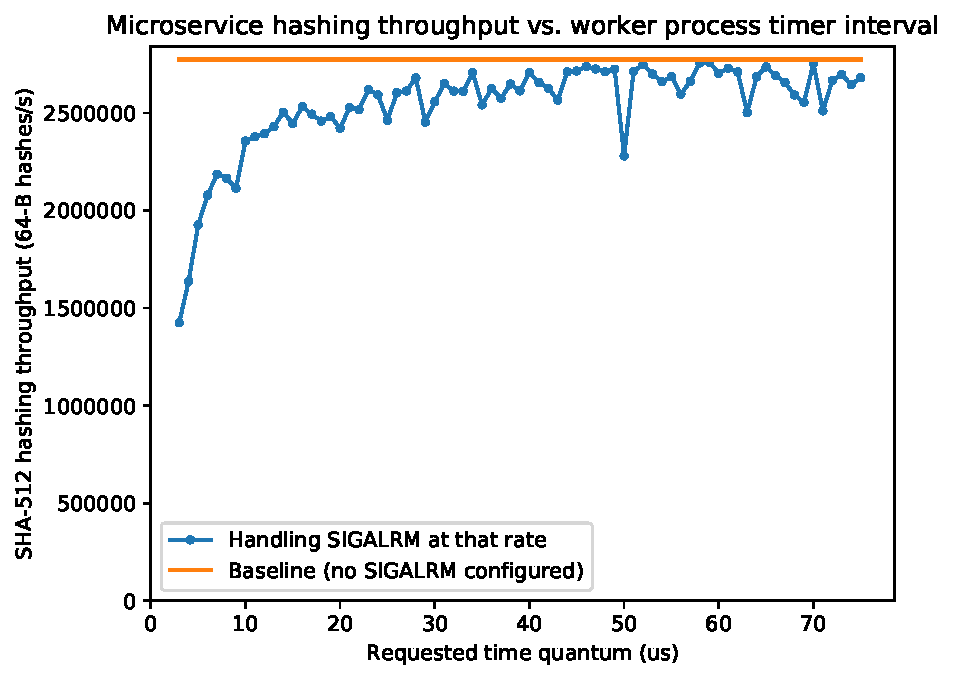
\includegraphics[width=\columnwidth]{figs/2018-02-02-evaluation_quantum-hasher_throughput-throughput}
\caption{Effect of \texttt{SIGALRM} quantum on hashing tput.}
\label{fig:hashtput}
\end{figure}
